\chapter{Project Setup \& Planning}

\section{Sie sind in der Lage, begründet darzulegen, worauf es bei dem Projekt-Setup ankommt.}

Definition Projekt:
\begin{itemize}
	\item Ein Projekt ist ein zeitlich begrenztes Vorhaben mit einem definierten Anfang und Ende.
	\item Um ein System/Produkt/Service zu erstellen oder anzupassen.
	\item Ein Projekt ist eine komplexe Aufgabe, welches einer Organisation bedarf.
\end{itemize}

Ein Projekt durchläuft verschiedene Projektphasen. Dabei tauchen viele Fragen auf, wie: Was ist das Problem? Wie Sehen die Prozesse aus? (siehe Abbildung \ref{fig:projekt-phasen-herauserforderungen})  Daher ist ein gutes Projekt-Setup notwendig und sollte folgendes umfassen:

\begin{itemize}
	\item Zeitrahmen
	\item Projektziele klar und eindeutig formulieren
	\item Projektresultate präzise und vollständig formulieren
	\item Meilensteine definieren
	\item Aufwand- und Ressourcenplanung
\end{itemize}

\begin{figure}[h!]
\centering
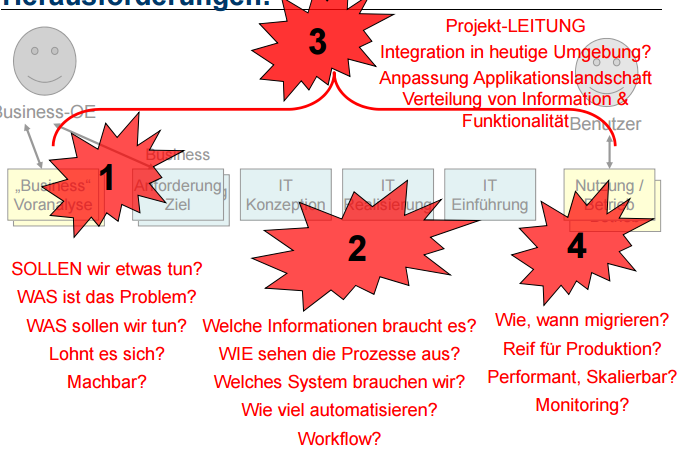
\includegraphics[width=0.7\linewidth]{fig/projekt-phasen-herauserforderungen}
\caption{Projekt-Phasen Herauserforderungen}
\label{fig:projekt-phasen-herauserforderungen}
\end{figure}

\section{Sie können erläutern, was ein Projektziel ist und sind in der Lage, anhand einer Situationsbeschreibung korrekte Projektziele zu definieren.}

Projekt-Ziele beschreiben was man mit dem Projekt will. Folgende Fragen führen zu Projekt-Zielen:
\begin{itemize}
	\item Was soll erreicht werden?
	\item Welche Eigenschaften soll der Endzustand haben?
	\item Was ist nach dem Projekt anders - besser! - als vorher?
\end{itemize}
Projekt-Ziele sollten \textbf{messbar} und \textbf{beurteilbar} sein jedoch keine Lösung aufzeigen. Tipp: Zuerst Resultate beschreiben und danach die Ziele! Ein Ziel beschreibt den \textbf{Zustand} wie es nach dem Projekt sein sollte. Fallstricke: Oft werden Resultate oder Ergebnisse als Ziele beschrieben.

\section{Sie vermögen den Unterschied zwischen Projekt-Zielen und Projekt-Ergebnissen zu erklären.}

Projekt-Ergbenisse und Projekt-Resultate werden als Synonyme gehandelt. Von den Projekt-Zielen bricht man die Hauptresultate herunter, diese kann man durch Teilresultate noch detaillieren und daraus entstehen die konkreten Arbeitspakete.
Die Resultate sind die Ergebnisse die ein Projekt erzeugt. Resultate sind kein Aktivitäten (Nicht das Durchführen eines Workshops ist interessant, sondern z.B. die daraus hervorgegangenen Anforderungen.). Die Resultate braucht man während des ganzen Projektes (Aufwandschätzung, Controlling, Reporting).

Ergebnisse in Softwareprojekten lassen sich fast immer in folgende Kategorien unterteilen (das Ergebnisraster):

\begin{enumerate}
	\item Applikationssoftware
	\item Applikationsdokumentation
	\item Prozesse
	\item Migration
	\item Rollout
	\item Projektmanagement-Ergebnisse
\end{enumerate}